\documentclass[dvipdfmx, 11pt, a4paper]{jsbook}

\usepackage{blindtext}
\usepackage[dvipdfmx]{graphicx}
\usepackage{natbib}

\newcounter{descriptcount}

\title{タイトル}
\date{build date: \today}
\author{著者}

\begin{document}
\maketitle
\tableofcontents
\bibliographystyle{jecon}

\chapter{hoge}

\blindtext

\section{表}


\LaTeX による表(表\ref{table:label_here})。

\begin{table}[hbtp]
  \caption{Caption here}
  \label{table:label_here}
  \centering
  \begin{tabular}{lcr}
    \hline
    列A  & 列B  &  列C  \\
    \hline \hline
    hoge  & fugar  & piyo \\
    foo  & bar  & baz \\
    \hline
  \end{tabular}
\end{table}


\blindtext

\subsection{引用方法}
\begin{description}
  \item[\texttt{\textbackslash cite}]\cite{doe2021-my-excelent} showed hoge
  \item[\texttt{\textbackslash citep}]Recent research \citep{doe2021-my-excelent} showed that
  \item[texttt{\textbackslash citealt}]\citealt{doe2021-my-excelent}
  \item[texttt{\textbackslash citealp}]\citealp{doe2021-my-excelent}
\end{description}

\clearpage

\subsection{図の挿入}

\begin{figure}[h]
\centering
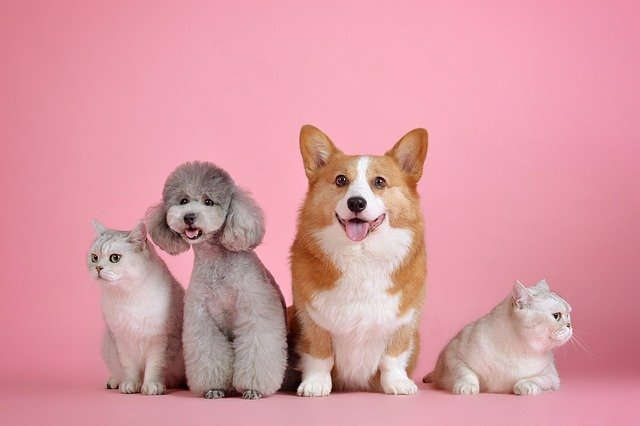
\includegraphics[scale=0.3]{figs/pets.jpg}
\caption{Cute pets}
\label{fig:pets}
\end{figure}


\section{piyo}

\blindtext

\chapter{foo}

\blindtext

\section{bar}

\blindtext

\section{baz}

\blindtext

\bibliography{references}

\end{document}
